%\documentclass[journal ]{new-aiaa}
\documentclass[conf]{new-aiaa} % for conference papers
\usepackage[utf8]{inputenc}
\usepackage{textcomp}

\usepackage{graphicx}
\usepackage{amsmath}
\usepackage[version=4]{mhchem}
\usepackage{siunitx}
\usepackage{longtable,tabularx}
\setlength\LTleft{0pt}

\title{Design and Analysis of Ram/Scramjet Engine}

\author{Stanley M. Porembski \footnote{Arizona State University Undergraduate Student, Aerospace Engineering (Autonomous Vehicle Systems).}}
\affil{Arizona State University Ira A. Schools of Engineering, Tempe, AZ, 85281}

\begin{document}

\maketitle

\begin{abstract}
These instructions give you guidelines for preparing papers for AIAA Technical Journals using \LaTeX{}. If you previously prepared an AIAA Conference Paper using the Meetings Papers Template, you may submit using the Meetings Papers Template so long as the text is double-spaced.  Carefully follow the journal paper submission process in Sec.~II of this document. Keep in mind that the electronic file you submit will be formatted further at AIAA. This first paragraph is formatted in the abstract style. Abstracts are required for regular, full-length papers and express articles. Be sure to define all symbols used in the abstract, and do not cite references in this section. The footnote on the first page should list the Job Title and AIAA Member Grade (if applicable) for each author.
\end{abstract}


\section*{Nomenclature}

\noindent(Nomenclature entries should have the units identified)

{\renewcommand\arraystretch{1.0}
\noindent\begin{longtable*}{@{}l @{\quad=\quad} l@{}}
    $a_j$ & speed of sound for state $j$ \\
    $A$ & area \\
    $c_p$ & specific heat \\
    $M_j$ & mach number for state $j$ \\
    $p_j$ & static pressure for state $j$ \\
    $p_{tj}$ & total pressure for state $j$ \\
    $R$ & gas constant of air \\
    $s$ & specific entropy \\
    $T_j$ & static temperature for state $j$ \\
    $T_{tj}$ & total temperature for state $j$ \\
    $V_j$ & flow velocity for state $j$ \\
    $z$ & flight altitude \\
    $z^*$ & reference altitude \\
    $\eta$ & efficiency \\
    $\gamma$ & ratio of specific heats \\
\multicolumn{2}{@{}l}{Subscripts} \\
    1 & free stream conditions \\
    2 & inlet/diffuser conditions \\
    3 & combusor conditions \\
    e & nozzle flow conditions \\
    4 & external flow conditions \\
    s & conditions at Earth's surface
\end{longtable*}}


\section{Introduction}
\lettrine{T}{he} primary focus of this project was to develop an analysis tool for studies of non-ideal ramjet propulsion performance. This tool was developed using FORTRAN for the non-ideal ramjet propulsion system with a converging-only fixed-geometry nozzle in Fig. \ref{fig:propsys}.

\begin{figure}[hbt!]
\centering
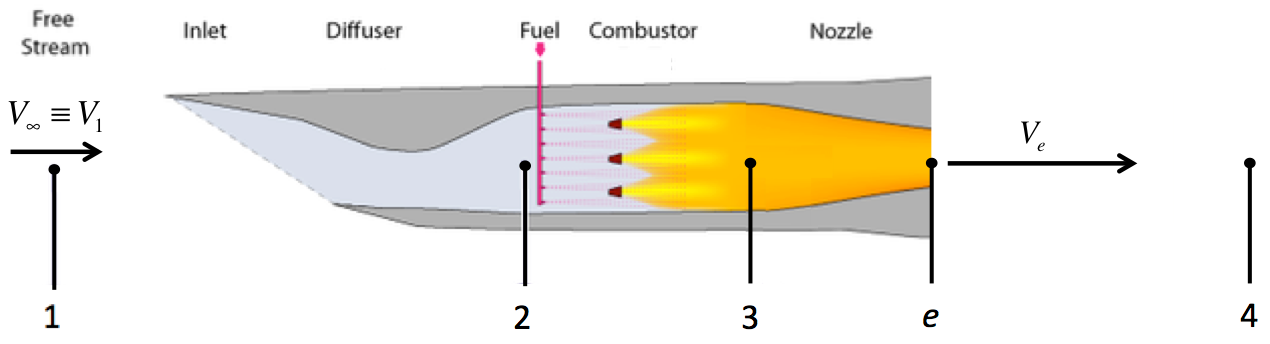
\includegraphics[width=0.75\textwidth]{media/the_ramjet.png}
\caption{\label{fig:propsys} The Ramjet Propulsion System}
\end{figure}

To analyze the ramjet, the analysis tool 

\begin{table}[hbt!]
\caption{\label{tab:table1} Parametric Analysis Tool Inputs}
\centering
\begin{tabular}{lcc}
\hline
Name& Variable& Units\\\hline
Flight Altitude& $z$& m\\
Flight Mach Number& $M_1$\\
Inlet/Diffuser Efficiency& $\eta_d$\\
Diffuser Exit Mach Number& $M_2$\\
Combustor Exit Max Allowable Total Temperature& $(T_{t3})_{max}$& K\\
Chosen Fuel Heating Value& $q_f$& MJ/kg\\
Nozzle Efficiency& $\eta_n$\\
Nozzle Exit Area& $A_e$& $m^2$\\
\hline
\end{tabular}
\end{table}


\section{Theory}
The

\section{Procedures}
The

\subsection{State 1: Free Stream}
The

\subsection{State 2: Inlet/Diffuser}
The

\subsection{State 3: Combustor}
The

\subsection{State 4: Internal Converging Nozzle Flow}
The

\subsection{State 5: External Flow Past Nozzle Exit}
The

\subsection{Ram/Scramjet Performance Parameters}
The


\section{Results}
The

\subsection{Part A: \textit{T-s} Diagrams for Validation Cases}
The

\begin{figure}[hbt!]
\centering
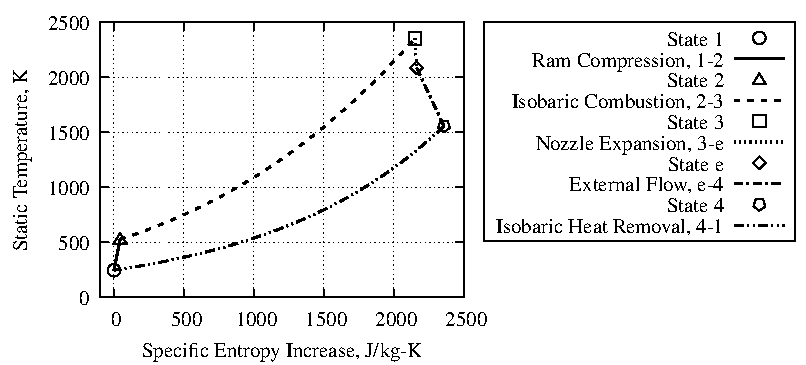
\includegraphics[]{media/ts_plot_files/TS_plot_for_case_7.pdf}
\caption{\label{fig:partavalida} Validation Case A}
\end{figure}
The

\begin{figure}[hbt!]
\centering
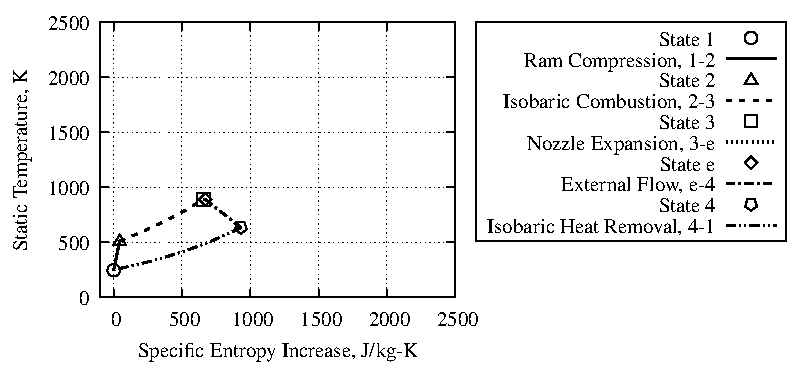
\includegraphics[]{media/ts_plot_files/TS_plot_for_case_8.pdf}
\caption{\label{fig:partavalidb} Validation Case B}
\end{figure}
The

\subsection{Part B: Atmospheric Model Validation}
The

\begin{figure}[hbt!]
\centering
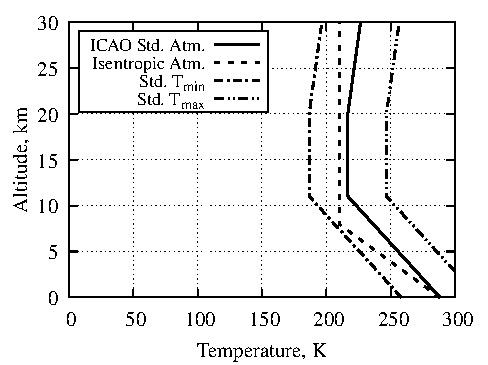
\includegraphics[]{media/atmosphere_validation_files/ICAO_vs_ISEN_temperature.pdf}
\caption{\label{fig:partbtemp} ICAO Standard Atmosphere vs Isentropic Model (Temperature)}
\end{figure}
The

\begin{figure}[hbt!]
\centering
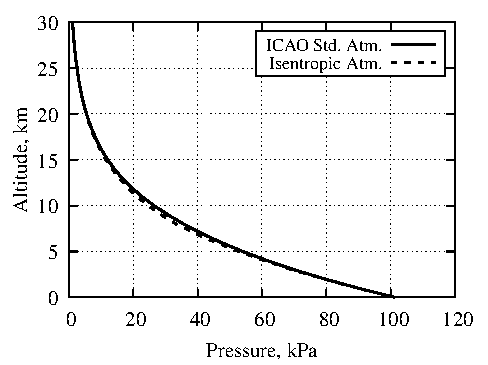
\includegraphics[]{media/atmosphere_validation_files/ICAO_vs_ISEN_pressure.pdf}
\caption{\label{fig:partbpres}ICAO Standard Atmosphere vs Isentropic Model (Pressure)}
\end{figure}
The

\subsection{Part C: Effect of Flight Mach Number}
The

\subsubsection{Overall Efficiency}
The

\begin{figure}[hbt!]
\centering
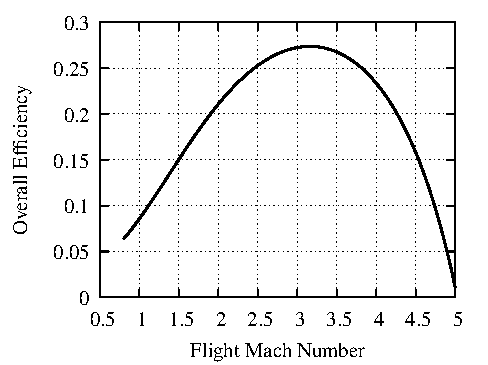
\includegraphics[]{media/performance_parameter_files/part_c_eta_o.pdf}
\caption{\label{fig:partcetao} Overall Efficiency vs Flight Mach Number}
\end{figure}
The

\subsubsection{Total Thrust}
The

\begin{figure}[hbt!]
\centering
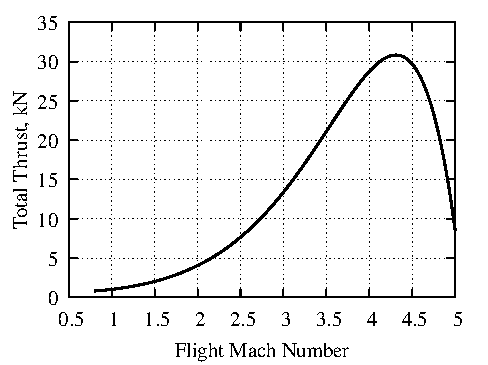
\includegraphics[]{media/performance_parameter_files/part_c_T.pdf}
\caption{\label{fig:partct} Total Thrust vs Flight Mach Number}
\end{figure}
The

\subsubsection{Thrust Specific Fuel Consumption}
The

\begin{figure}[hbt!]
\centering
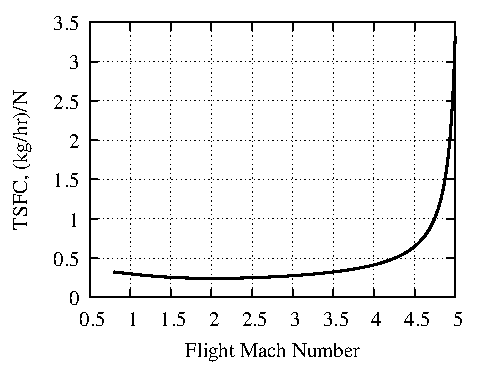
\includegraphics[]{media/performance_parameter_files/part_c_TSFC.pdf}
\caption{\label{fig:partctsfc} TSFC vs Flight Mach Number}
\end{figure}
The

\subsection{Part D: Effect of Flight Altitude}
The

\subsubsection{Overall Efficiency}
The

\begin{figure}[hbt!]
\centering
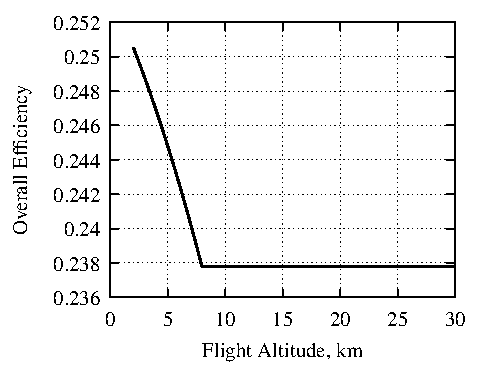
\includegraphics[]{media/performance_parameter_files/part_d_eta_o.pdf}
\caption{\label{fig:partdetao} Overall Efficiency vs Flight Altitude}
\end{figure}
The

\subsubsection{Total Thrust}
The

\begin{figure}[hbt!]
\centering
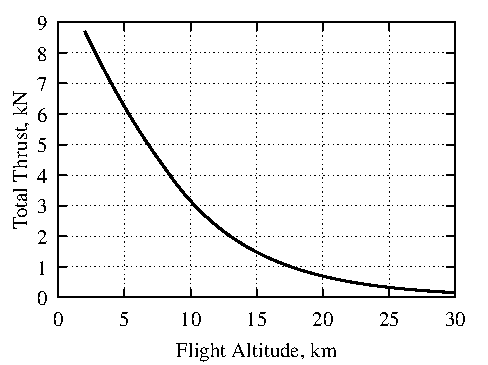
\includegraphics[]{media/performance_parameter_files/part_d_T.pdf}
\caption{\label{fig:partdt} Total Thrust vs Flight Altitude}
\end{figure}
The

\subsubsection{Thrust Specific Fuel Consumption}
The

\begin{figure}[hbt!]
\centering
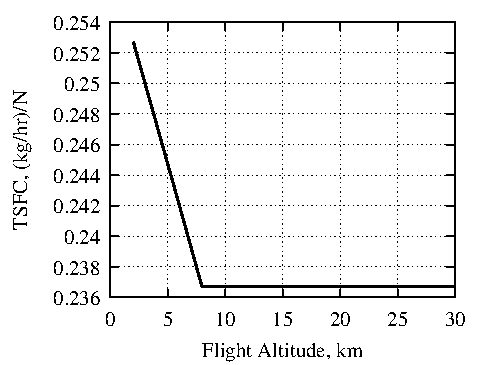
\includegraphics[]{media/performance_parameter_files/part_d_TSFC.pdf}
\caption{\label{fig:partdtsfc} TSFC vs Flight Altitude}
\end{figure}
The

\subsection{Part E: Optimizing TSFC}
The

\subsection{Part F: Effect of Inlet/Diffuser Efficiency}
The

\subsubsection{Overall Efficiency}
The

\begin{figure}[hbt!]
\centering
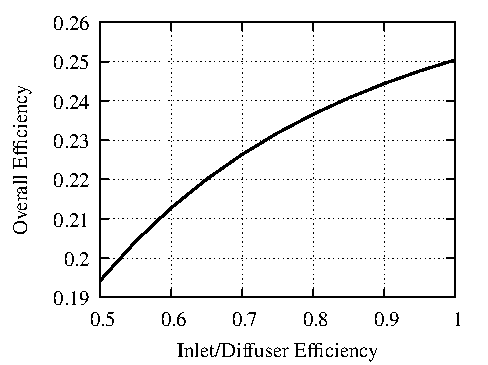
\includegraphics[]{media/performance_parameter_files/part_f_eta_o.pdf}
\caption{\label{fig:partfetao} Overall Efficiency vs Inlet/Diffuser Efficiency}
\end{figure}
The

\subsubsection{Total Thrust}
The

\begin{figure}[hbt!]
\centering
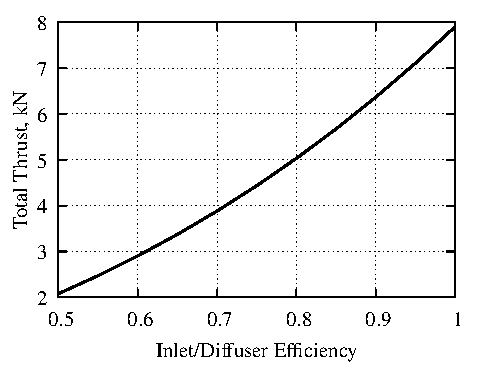
\includegraphics[]{media/performance_parameter_files/part_f_T.pdf}
\caption{\label{fig:partft} Total Thrust vs Inlet/Diffuser Efficiency}
\end{figure}
The

\subsubsection{Thrust Specific Fuel Consumption}
The

\begin{figure}[hbt!]
\centering
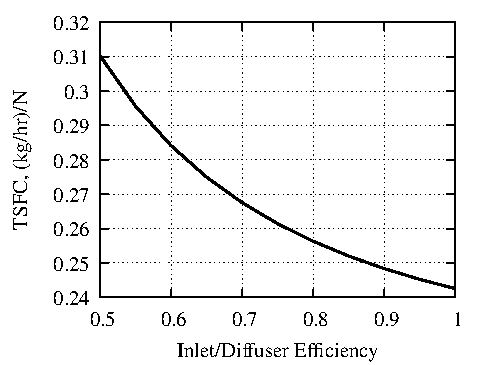
\includegraphics[]{media/performance_parameter_files/part_f_TSFC.pdf}
\caption{\label{fig:partftsfc} TSFC vs Inlet/Diffuser Efficiency}
\end{figure}
The

\subsection{Part G: Effect of Nozzle Efficiency}
The

\subsubsection{Overall Efficiency}
The

\begin{figure}[hbt!]
\centering
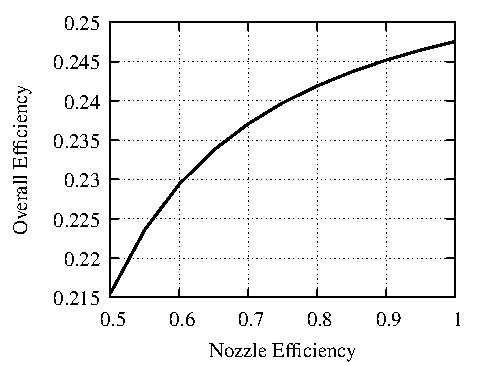
\includegraphics[]{media/performance_parameter_files/part_g_eta_o.pdf}
\caption{\label{fig:partgetao} Overall Efficiency vs Nozzle Efficiency}
\end{figure}
The

\subsubsection{Total Thrust}
The

\begin{figure}[hbt!]
\centering
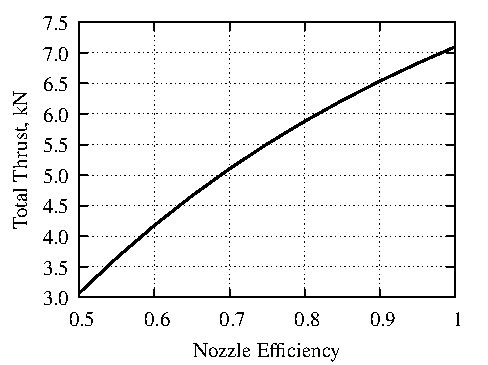
\includegraphics[]{media/performance_parameter_files/part_g_T.pdf}
\caption{\label{fig:partgt} Total Thrust vs Nozzle Efficiency}
\end{figure}
The

\subsubsection{Thrust Specific Fuel Consumption}
The

\begin{figure}[hbt!]
\centering
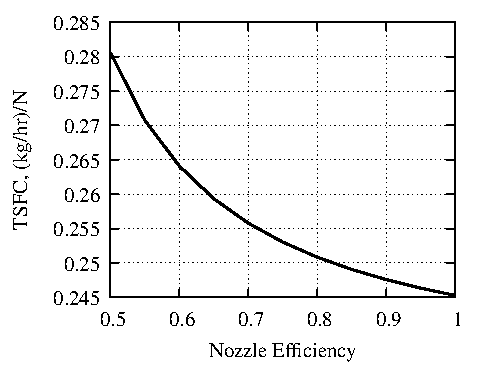
\includegraphics[]{media/performance_parameter_files/part_g_TSFC.pdf}
\caption{\label{fig:partgtsfc} TSFC vs Nozzle Efficiency}
\end{figure}
The

\subsection{Part H: Effect of \texorpdfstring{\textit{$M_2$}}{M2}}
The

\subsubsection{Overall Efficiency}
The

\begin{figure}[hbt!]
\centering
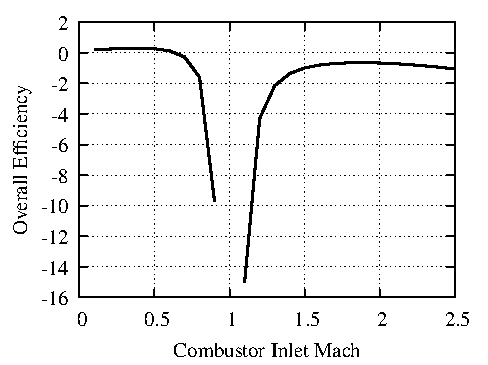
\includegraphics[]{media/performance_parameter_files/part_h_eta_o.pdf}
\caption{\label{fig:parthetao} Overall Efficiency vs \texorpdfstring{\textit{$M_2$}}{M2}}
\end{figure}
The

\subsubsection{Total Thrust}
The

\begin{figure}[hbt!]
\centering
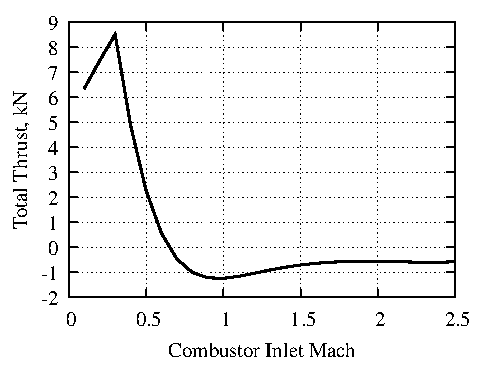
\includegraphics[]{media/performance_parameter_files/part_h_T.pdf}
\caption{\label{fig:partht} Total Thrust vs \texorpdfstring{\textit{$M_2$}}{M2}}
\end{figure}
The

\subsubsection{Thrust Specific Fuel Consumption}
The

\begin{figure}[hbt!]
\centering
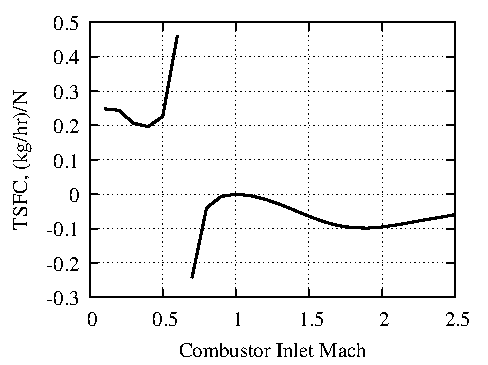
\includegraphics[]{media/performance_parameter_files/part_h_TSFC.pdf}
\caption{\label{fig:parthtsfc} TSFC vs \texorpdfstring{\textit{$M_2$}}{M2}}
\end{figure}
The

\subsection{Part I: Optimzed Ram/Scramjet Propulsion System}
The

\begin{figure}[hbt!]
\centering
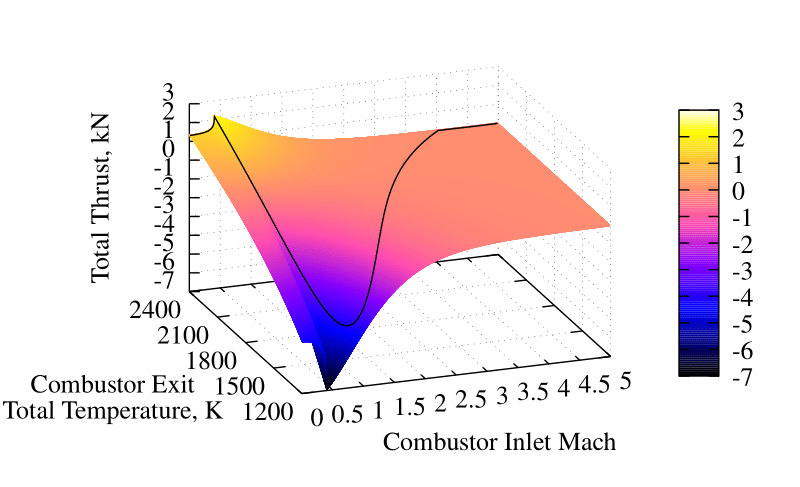
\includegraphics[]{media/propulsion_design_files/total_thrust_plot.pdf}
\caption{\label{fig:partithrust} Total Thrust}
\end{figure}
The

\begin{figure}[hbt!]
\centering
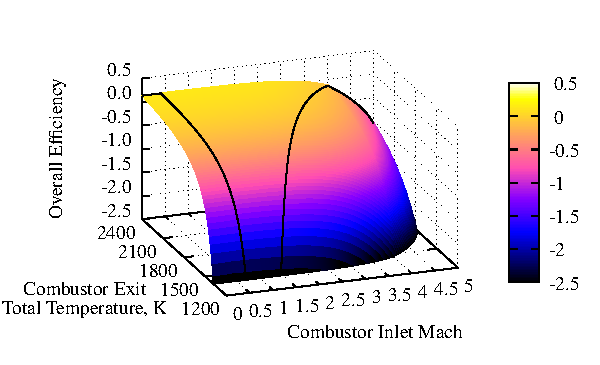
\includegraphics[]{media/propulsion_design_files/eta_o_plot.pdf}
\caption{\label{fig:partietao} Overall Efficiency}
\end{figure}
The


\section{Conclusion}
Although a conclusion may review the main points of the paper, it must not replicate the abstract. A conclusion might elaborate on the importance of the work or suggest applications and extensions. Do not cite references in the conclusion. Note that the conclusion section is the last section of the paper to be numbered. The appendix (if present), funding information, other acknowledgments, and references are listed without numbers.


\section*{Appendix}

\subsection{Universal Module Code}

\begin{verbatim}
    module universal_module
    use, intrinsic :: iso_fortran_env, only: sp=>real32, dp=>real64
    implicit none

    public pi

    real(dp), parameter :: pi = 4.0*atan(1.0)

    contains

    subroutine linspace(from, to, array)
        implicit none
        real(dp), intent(in) :: from, to
        real(dp), intent(out) :: array(:)
        real(dp) :: range
        integer :: n, i
        n = size(array)
        range = to - from
    
        if (n == 0) return
    
        if (n == 1) then
            array(1) = from
            return
        end if
        
        do i=1, n
            array(i) = from + range * (i - 1) / (n - 1)
        end do
    end subroutine linspace

    subroutine write_2_arrays_to_file(filename, array1, array2)
        implicit none

        character(len=*), intent(in) :: filename
        real(dp), intent(in) :: array1(:), array2(:)
        integer :: i, n, unit
    
        ! Ensure both arrays have the same size
        n = size(array1)
        if (n /= size(array2)) then
            print *, 'Error: Arrays must have the same size.'
            stop
        end if
    
        ! Open the file for writing
        open (newunit=unit, file=filename, status='replace', action='write')
    
        ! Write the data to the file
        do i = 1, n
            write(unit, '(F20.10, ",", F20.10)') array1(i), array2(i)
        end do
    
        ! Close the file
        close(unit)
    end subroutine write_2_arrays_to_file

    subroutine write_3_arrays_to_file(filename, array1, array2, array3)
        implicit none

        character(len=*), intent(in) :: filename
        real(dp), intent(in) :: array1(:), array2(:), array3(:)
        integer :: i, n, unit
    
        ! Ensure both arrays have the same size
        n = size(array1)
        if (n /= size(array2)) then
            print *, 'Error: Arrays must have the same size.'
            stop
        end if
    
        ! Open the file for writing
        open (newunit=unit, file=filename, status='replace', action='write')
    
        ! Write the data to the file
        do i = 1, n
            write(unit, '(F20.10, ",", F20.10, ",", F20.10)') &
                  array1(i), array2(i), array3(i)
        end do
    
        ! Close the file
        close(unit)
    end subroutine write_3_arrays_to_file

    subroutine write_4_arrays_to_file(filename, array1, array2, array3, array4)
        implicit none

        character(len=*), intent(in) :: filename
        real(dp), intent(in) :: array1(:), array2(:), array3(:), array4(:)
        integer :: i, n, unit
    
        ! Ensure both arrays have the same size
        n = size(array1)
        if (n /= size(array2)) then
            print *, 'Error: Arrays must have the same size.'
            stop
        end if
    
        ! Open the file for writing
        open (newunit=unit, file=filename, status='replace', action='write')
    
        ! Write the data to the file
        do i = 1, n
            write(unit, '(F20.10, ",", F20.10, ",", F20.10, ",", F20.10)') &
                  array1(i), array2(i), array3(i), array4(i)
        end do
    
        ! Close the file
        close(unit)
    end subroutine write_4_arrays_to_file

    function count_lines(filename,nheadder) result(nlines)
        implicit none

        character(len=*), intent(in) :: filename
        integer :: nlines, nheadder, i, iounit
        real :: dummy1, dummy2, dummy3

        nlines = 0

        open (newunit=iounit, file=filename, status='old', action='read')
        do i = 1, nheadder
            read (iounit,*)
        end do
        do
            read (iounit,*, end=10) dummy1, dummy2, dummy3
            nlines = nlines + 1
        end do

10      close (iounit)
        rewind (iounit)
    end function count_lines

    function split_data(filename,nheadder,ncolumn) result(data_matrix)
        implicit none

        character(len=*), intent(in) :: filename
        real, allocatable :: data_matrix(:,:)
        integer :: nheadder, ncolumn, nlines, iounit, i

        nlines = count_lines(filename,nheadder)

        allocate(data_matrix(nlines,ncolumn))

        open (newunit=iounit, file=filename, status='old', action='read')
        if (nheadder /= 0) then
            do i = 1, nheadder
                read (iounit,*)
            end do
        end if
        do i = 1,nlines
            read (iounit,*) data_matrix(i,:)
        end do

        close (iounit)
        rewind (iounit)
    end function split_data

    function quadratic_equation_rr(a,b,c) result(x)
        implicit none

        real(dp), intent(in) :: a, b, c
        real(dp) :: discriminant
        real(dp), allocatable :: x(:)

        discriminant = b**2 - 4*a*c

        if (discriminant > 0) then
            allocate(x(2))
            x(1) = (-b + sqrt(discriminant)) / (2 * a)
            x(2) = (-b - sqrt(discriminant)) / (2 * a)
        else if (discriminant == 0) then
            allocate(x(1))
            x = -b / (2 * a)
        else
            allocate(x(0))
        end if
    end function quadratic_equation_rr
end module universal_module
\end{verbatim}

\subsection{Module 1 Code}

\begin{verbatim}
module module_1
    use universal_module
    use, intrinsic :: iso_fortran_env, only: sp=>real32, dp=>real64
    implicit none

    real(dp), parameter :: Ts = 288                                     ! K
    real(dp), parameter :: ps = 101.3                                   ! kPa
    real(dp), parameter :: R_1 = 286.9                                  ! J/kg-K
    real(dp), parameter :: gamma_1 = 1.40
    real(dp), parameter :: z_star = 8404                                ! m

    contains

    function M1_pressure_coefficient() result(cp)
        ! Pressure Coefficient for states 1 & 2
        implicit none

        real(dp) :: cp

        cp = gamma_1 * R_1 / (gamma_1 - 1)                              ! J/kg-K
    end function M1_pressure_coefficient

    function M1_isentropic_atmos_model(z) result(Temp_n_pres)
        ! Isentropic model of the atmosphere
        implicit none

        real(dp), intent(in) :: z
        real(dp) :: T1_Ts, T1, p1, Temp_n_pres(2)

        if (z <= 7958._dp) then
            T1_Ts = (1 - (gamma_1 - 1) * (z / z_star) / gamma_1)
            T1 = Ts * T1_Ts
            p1 = ps * T1_Ts**(gamma_1 / (gamma_1 - 1))
        else
            T1 = 210
            p1 = 33.6 * exp(-(z - 7958) / 6605)
        end if

        Temp_n_pres = [T1,p1]
    end function M1_isentropic_atmos_model

    function M1_total_to_static_relations(M1,T1,p1) result(out)
        ! Total to static relations for state 1
        implicit none

        real(dp), intent(in) :: M1, T1, p1
        real(dp) :: Tt1_T1, pt1_p1, out(2)
        
        Tt1_T1 = 1 + (gamma_1 - 1) / 2 * M1**2
        pt1_p1 = Tt1_T1**(gamma_1 / (gamma_1 - 1))

        out = [Tt1_T1 * T1,pt1_p1 * p1]
    end function M1_total_to_static_relations

    function M1_speed_of_sound(T,gamma,R) result(a)
        ! Speed of sound calculations for all states
        implicit none

        real(dp), intent(in) :: T, gamma, R
        real(dp) :: a

        a = sqrt(gamma * R * T)
    end function M1_speed_of_sound

    function M1_flow_speed(M,a) result(V)
        ! Air flow speed calculations for all states
        implicit none

        real(dp), intent(in) :: M, a
        real(dp) :: V
        
        V = M * a
    end function M1_flow_speed

    function M1_all_function(z,M1) result(M1_output_matrix)
        ! Module 1 function that combines all previous functions
        ! and outputs required data for state 1
        implicit none

        real(dp), intent(in) :: z, M1
        real(dp) :: Temp_n_pres(2), T2S_relations(2)
        real(dp) :: M1_output_matrix(7)
        real(dp) :: T1, p1, Tt1, pt1, cp1, a1, V1

        Temp_n_pres = M1_isentropic_atmos_model(z)
        T1 = Temp_n_pres(1)
        p1 = Temp_n_pres(2)
        
        T2S_relations = M1_total_to_static_relations(M1,T1,p1)
        Tt1 = T2S_relations(1)
        pt1 = T2S_relations(2)
        cp1 = M1_pressure_coefficient()

        a1 = M1_speed_of_sound(T1,gamma_1,R_1)
        V1 = M1_flow_speed(M1,a1)

        M1_output_matrix = [T1,p1,Tt1,pt1,cp1,a1,V1]
    end function M1_all_function
end module module_1
\end{verbatim}

\subsection{Module 2 Code}

\begin{verbatim}
    module module_2
    use universal_module
    use module_1
    use, intrinsic :: iso_fortran_env, only: sp=>real32, dp=>real64
    implicit none

    contains

    function M2_total_to_static_relations(Tt1,p1,M1,M2,eta_d) result(out)
        ! Total to static relaitons for state 2
        implicit none

        real(dp), intent(in) :: Tt1, p1, M1, M2, eta_d
        real(dp) :: Tt2, T2, pt2, p2, Tt2_T2, out(4)

        Tt2 = Tt1
        Tt2_T2 = (1 + (gamma_1 - 1) / 2 * M2**2)
        T2 = Tt2 / Tt2_T2
        pt2 = p1 * (1 + eta_d * (gamma_1 - 1) / 2 * M1**2)**(gamma_1 / &
                                                            (gamma_1 - 1))
        p2 = pt2 / (Tt2_T2**(gamma_1 / (gamma_1-1)))

        out = [T2,Tt2,p2,pt2]
    end function M2_total_to_static_relations

    function M2_entropy_increase(Tt1,Tt2,pt1,pt2) result(delta_s)
        ! Entropy increase from state 1 to 2
        implicit none

        real(dp), intent(in) :: Tt1, Tt2, pt1, pt2
        real(dp) :: cp, delta_s

        cp = M1_pressure_coefficient()
        delta_s = cp * log(Tt2 / Tt1) - R_1 * log(pt2 / pt1)

    end function M2_entropy_increase
    
    function M2_all_function(Tt1,p1,pt1,M1,M2,eta_d) result(M2_output_matrix)
        ! Module 2 function that combines all previous functions
        ! and outputs required data for state 2
        implicit none

        real(dp), intent(in) :: Tt1, p1, pt1, M1, M2, eta_d
        real(dp) :: T2S_relations(4)
        real(dp) :: M2_output_matrix(8)
        real(dp) :: T2, Tt2, p2, pt2, delta_s12, cp2, a2, V2

        T2S_relations = M2_total_to_static_relations(Tt1,p1,M1,M2,eta_d)
        T2 = T2S_relations(1)
        Tt2 = T2S_relations(2)
        p2 = T2S_relations(3)
        pt2 = T2S_relations(4)

        delta_s12 = M2_entropy_increase(Tt2,Tt2,pt1,pt2)

        cp2 = M1_pressure_coefficient()
        a2 = M1_speed_of_sound(T2,gamma_1,R_1)
        V2 = M1_flow_speed(M2,a2)

        M2_output_matrix = [Tt2,T2,pt2,p2,cp2,a2,V2,delta_s12]
    end function M2_all_function
end module module_2
\end{verbatim}

\subsection{Module 3 Code}

\begin{verbatim}
    module module_3
    use universal_module
    use module_2
    use, intrinsic :: iso_fortran_env, only: sp=>real32, dp=>real64
    implicit none

    real(dp), parameter :: R_3 = 286.9                                  ! J/kg-K
    real(dp), parameter :: gamma_3 = 1.30
    real(dp), parameter :: cp_a = 986
    real(dp), parameter :: cp_b = 0.179

    contains

    function M3_pressure_coefficient(T) result(cp)
        ! Pressure Coefficient for states 3, e, & 4
        implicit none

        real(dp), intent(in) :: T
        real(dp) :: cp

        cp = cp_a + (cp_b * T)                                          ! J/kg-K
    end function M3_pressure_coefficient

    function M3_thermal_choking(Tt2,M2) result(Tt3_choked)
        ! Calculations for thermally choked T3 value
        implicit none

        real(dp), intent(in) :: Tt2, M2
        real(dp) :: Tt3_choked

        Tt3_choked = Tt2 * ((1 + gamma_3 * M2**2)**2 / (2 * (gamma_3 + 1) * &
         M2**2)  &
                     * (1 + 0.5 * (gamma_3 - 1) * M2**2)**(-1))

    end function M3_thermal_choking

    function M3_combustor_conditions(Tt2,Tt3_max,M2) result(out_matrix)
        ! Total temperature and mach for state 3
        implicit none

        real(dp), intent(in) :: Tt2, Tt3_max, M2
        real(dp), allocatable :: Mach(:)
        real(dp) :: Tt3, Tt3_choked, out_matrix(2)
        real(dp) :: a_Mod3, b_Mod3, c_Mod3, c_mach, M3
        integer :: i

        Tt3_choked = M3_thermal_choking(Tt2,M2)

        if (Tt3_choked < Tt3_max) then
            M3 = 1
            Tt3 = Tt3_choked
        else
            Tt3 = Tt3_max
            c_mach = M2**2 * Tt3 * (1 + 0.5 * (gamma_3 - 1) * M2**2) &
                     / (Tt2 * (1 + gamma_3 * M2**2)**2)
            a_Mod3 = c_mach * gamma_3**2 - (gamma_3 - 1) / 2
            b_Mod3 = 2 * c_mach * gamma_3 - 1
            c_Mod3 = c_mach
            Mach = sqrt(quadratic_equation_rr(a_Mod3,b_Mod3,c_Mod3))

            do i = 1,size(Mach)
                if (M2 < 1 .and. Mach(i) <= 1) then
                    M3 = mach(i)
                else if (M2 > 1 .and. Mach(i) >= 1) then
                    M3 = Mach(i)
                else
                    M3 = Mach(i)
                end if
            end do
        end if

        out_matrix = [M3,Tt3]
    end function M3_combustor_conditions

    function M3_heat_added(Tt2,Tt3) result(q23)
        ! Heat per unit mass added in the combustor
        implicit none

        real(dp), intent(in) :: Tt2, Tt3
        real(dp) :: q23

        q23 = cp_a * (Tt3 - Tt2) + 0.5 * cp_b * (Tt3**2 - Tt2**2)
    end function M3_heat_added

    function M3_total_to_static_relations(Tt3,p2,M3) result(Temp_n_pres)
        ! Total to static relations for state 3
        implicit none

        real(dp), intent(in) :: Tt3, p2, M3
        real(dp) :: p3, pt3, T3, Tt3_T3
        real(dp) :: Temp_n_pres(3)

        p3 = p2
        Tt3_T3 = 1 + 0.5 * (gamma_3 - 1) * M3**2
        T3 = Tt3 / Tt3_T3
        pt3 = p3 * Tt3_T3**(gamma_3 / (gamma_3 - 1))
        Temp_n_pres = [T3,p3,pt3]
    end function M3_total_to_static_relations

    function M3_entropy_increase(Tt2,Tt3,pt2,pt3,cp3) result(delta_s23)
        ! Entropy increase from state 2 to 3, and state 3 to e
        implicit none

        real(dp), intent(in) :: Tt2, Tt3, pt2, pt3, cp3
        real(dp) :: delta_s23

        delta_s23 = cp3 * log(Tt3 / Tt2) - R_3 * log(pt3 / pt2)
    end function M3_entropy_increase

    function M3_all_function(Tt2,Tt3_max,p2,pt2,M2,delta_s12,Tt3_in,cp3_in) &
         result(M3_output_matrix)
        ! Module 3 function that combines all previous functions
        ! and outputs required data for state 3
        implicit none

        real(dp), intent(in) :: Tt2, Tt3_max, p2, pt2, M2, delta_s12
        real(dp), optional :: Tt3_in, cp3_in
        real(dp) :: M3, q23, T3, Tt3, p3, cp3, pt3, a3, V3, delta_s23
        real(dp) :: delta_s13
        real(dp) :: comb_conditions(2), T2S_relaitons(3)
        real(dp) :: M3_output_matrix(9)

        comb_conditions = M3_combustor_conditions(Tt2,Tt3_max,M2)
        M3 = comb_conditions(1)

        if(present(Tt3_in)) then
            Tt3 = Tt3_in
        else
            Tt3 = comb_conditions(2)
        end if

        q23 = M3_heat_added(Tt2,Tt3) / 1e6

        T2S_relaitons = M3_total_to_static_relations(Tt3,p2,M3)
        T3 = T2S_relaitons(1)
        p3 = T2S_relaitons(2)
        pt3 = T2S_relaitons(3)

        if(present(cp3_in)) then
            cp3 = cp3_in
        else
            cp3 = M3_pressure_coefficient(T3)
        end if
        a3 = M1_speed_of_sound(T3,gamma_3,R_3)
        V3 = M1_flow_speed(M3,a3)

        delta_s23 = M3_entropy_increase(Tt2,Tt3,pt2,pt3,cp3)
        delta_s13 = delta_s12 + delta_s23

        M3_output_matrix = [Tt3,M3,q23,T3,p3,pt3,cp3,delta_s23,delta_s13]
    end function M3_all_function
end module module_3
\end{verbatim}

\subsection{Module 4 Code}

\begin{verbatim}
module module_4
    use universal_module
    use module_3
    use, intrinsic :: iso_fortran_env, only: sp=>real32, dp=>real64
    implicit none

    contains

    function M4_test_mach(p1,pt3,eta_n) result(M_prime)
        ! Test Mach number, M' calcualtion
        implicit none

        real(dp), intent(in) :: p1, pt3, eta_n
        real(dp) :: var1, M_prime

        var1 = 1 - (p1 / pt3)**((gamma_3 - 1) / gamma_3)
        M_prime = (2 * eta_n * var1 / ((gamma_3 - 1) * (1 - eta_n * var1)))**0.5

    end function M4_test_mach

    function M4_nozzle_choke_test(Tt3,p1,pt3,eta_n) result(nozzle_conditions)
        ! Test for nozzle choking, outputs total temperature, static pressure,
        ! and Mach at state e
        implicit none

        real(dp), intent(in) :: Tt3, p1, pt3, eta_n
        real(dp) :: Me, pe, Tte, M_prime, nozzle_conditions(3)

        Tte = Tt3
        M_prime = M4_test_mach(p1,pt3,eta_n)

        if (M_prime < 1) then
            Me = M_prime
            pe = p1
        else
            Me = 1
            pe = pt3 * (1 - ((gamma_3 - 1) / (gamma_3 + 1)) / eta_n)**& 
                       (gamma_3 / (gamma_3 - 1))
        end if

        nozzle_conditions = [Me,pe,Tte]
    end function M4_nozzle_choke_test

    function M4_total_to_static_relations(Tte,pe,Me) result(Temp_n_pres)
        ! Total to static relations for state e
        implicit none

        real(dp), intent(in) :: Tte, pe, Me
        real(dp) :: Tte_Te, pte_pe, Temp_n_pres(2)

        Tte_Te = 1 + 0.5 * (gamma_3 - 1) * Me**2
        pte_pe = Tte_Te**(gamma_3 / (gamma_3 - 1))

        Temp_n_pres = [Tte / Tte_Te, pe * pte_pe]
    end function M4_total_to_static_relations

    function M4_exit_mass_flux(Te,pe,Ve,Area_e) result(me_dot)
        ! Exit mass flux from nozzle
        implicit none

        real(dp), intent(in) :: Te, pe, Ve, Area_e
        real(dp) :: me_dot

        me_dot = pe * Ve * Area_e / (R_3 * Te)
    end function M4_exit_mass_flux

    function M4_all_function(Tt3,p1,pt3,eta_n,delta_s13,Area_e) &
             result(M4_output_matrix)
        ! Module 4 function that combines all previous functions
        ! and outputs required data for state e
        implicit none

        real(dp), intent(in) :: Tt3, p1, pt3, eta_n, delta_s13, Area_e
        real(dp) :: Me, pe, pte, Te, Tte, ae, cpe, Ve, me_dot
        real(dp) :: delta_s3e, delta_s1e
        real(dp) :: nozzle_choke(3), T2S_relations(2)
        real(dp) :: M4_output_matrix(11)

        nozzle_choke = M4_nozzle_choke_test(Tt3,p1,pt3,eta_n)
        Me = nozzle_choke(1)
        pe = nozzle_choke(2)
        Tte = nozzle_choke(3)

        T2S_relations = M4_total_to_static_relations(Tte,pe,Me)
        Te = T2S_relations(1)
        pte = T2S_relations(2)

        cpe = M3_pressure_coefficient(Te)
        ae = M1_speed_of_sound(Te,gamma_3,R_3)
        Ve = M1_flow_speed(Me,ae)
        me_dot = M4_exit_mass_flux(Te,pe,Ve,Area_e) * 1e3

        delta_s3e = M3_entropy_increase(Tt3,Te,Tte,pt3,pte)
        delta_s1e = delta_s13 + delta_s3e

        M4_output_matrix = [Me,pte,pe,Tte,Te,cpe,ae,Ve,me_dot, &
                            delta_s3e,delta_s1e]
    end function M4_all_function
end module module_4
\end{verbatim}

\subsection{Module 5 Code}

\begin{verbatim}
module module_5
    use universal_module
    use module_4
    use, intrinsic :: iso_fortran_env, only: sp=>real32, dp=>real64
    implicit none

    contains

    function M5_nozzle_external_efficiency(p1,pt3,eta_n) result(eta_n_ext)
        ! Nozzle external efficiency calculations
        implicit none

        real(dp), intent(in) :: p1,pt3,eta_n
        real(dp) :: M_prime, eta_n_ext

        M_prime = M4_test_mach(p1,pt3,eta_n)

        if (M_prime < 1) then
            eta_n_ext = 1
        else
            eta_n_ext = M_prime**(-0.3)
        end if
    end function M5_nozzle_external_efficiency

    function M5_total_to_static_relations(eta_n_ext,p1,pte,Tte) &
             result(output_array)
        ! Total to static relations for state 4
        implicit none

        real(dp), intent(in) :: eta_n_ext, p1, pte, Tte
        real(dp) :: Tt4, T4_Tt4, p4, pt4_p4, M4, output_array(5)

        Tt4 = Tte
        T4_Tt4 = 1 - eta_n_ext * (1 - (p1 / pte)**((gamma_3 - 1) / gamma_3))
        M4 = (2 * (T4_Tt4**(-1) - 1) / (gamma_3 - 1))**0.5
        p4 = p1
        pt4_p4 = (1 + 0.5 * (gamma_3 - 1) * M4**2)**(gamma_3 / (gamma_3 - 1))

        output_array = [Tt4,Tt4 * T4_Tt4,p4,p4 * pt4_p4,M4]
    end function M5_total_to_static_relations

    function M5_entropy_increase(Tt4,T4,Tte,pt4,pte) result(delta_se4)
        ! Entropy increase from state e to 4
        implicit none

        real(dp), intent(in) :: Tt4, T4, Tte, pt4, pte
        real(dp) :: cp, delta_se4

        cp =  M3_pressure_coefficient(T4)
        delta_se4 = cp * log(Tt4 / Tte) - R_3 * log(pt4 / pte)
    end function M5_entropy_increase

    function M5_all_function(p1,pt3,pte,Tte,eta_n,delta_s1e) &
             result(M5_output_array)
        ! Module 5 function that combines all previous functions
        ! and outputs required data for state 4
        implicit none

        real(dp), intent(in) :: p1, pt3, pte, Tte, eta_n, delta_s1e
        real(dp) :: eta_n_ext, T2S_relations(5)
        real(dp) :: M4, pt4, p4, Tt4, T4, cp4, a4, V4, delta_se4, delta_s14
        real(dp) :: M5_output_array(10)

        eta_n_ext = M5_nozzle_external_efficiency(p1,pt3,eta_n)
        
        T2S_relations = M5_total_to_static_relations(eta_n_ext,p1,pte,Tte)
        Tt4 = T2S_relations(1)
        T4 = T2S_relations(2)
        p4 = T2S_relations(3)
        pt4 = T2S_relations(4)
        M4 = T2S_relations(5)

        cp4 = M3_pressure_coefficient(T4)

        a4 = M1_speed_of_sound(T4,gamma_3,R_3)
        V4 = M1_flow_speed(M4,a4)

        delta_se4 = M5_entropy_increase(Tt4,T4,Tte,pt4,pte)
        delta_s14 = delta_s1e + delta_se4

        M5_output_array = [M4,pt4,p4,Tt4,T4,cp4,a4,V4,delta_se4,delta_s14]
    end function M5_all_function
end module module_5
\end{verbatim}

\subsection{Module 6 Code}

\begin{verbatim}
    module module_6
    use universal_module
    use module_5
    use, intrinsic :: iso_fortran_env, only: sp=>real32, dp=>real64
    implicit none

    real(dp), parameter :: g_acc = 9.8                                   ! m/s^2

    contains

    function M6_mass_and_fuel_calcualtions(q23,qf,me_dot) result(mass_array)
        ! Calculations for the inlet mass flux (m1_dot)
        ! and fuel-air mass ratio (f)
        implicit none

        real(dp), intent(in) :: q23, qf, me_dot
        real(dp) :: mi_dot, mf_dot, f, mass_array(3)

        mi_dot = me_dot / (1 + q23 / qf)
        mf_dot = me_dot - mi_dot
        f = mf_dot / mi_dot
        mass_array = [mi_dot,mf_dot,f]
    end function M6_mass_and_fuel_calcualtions

    function M6_thrust_calculations(mi_dot,mf_dot,f,Ve,V1,pe,p1,Area_e) &
             result(thrust_array)
        ! Calculations for jet thrust, pressure thrust, total thrust,
        ! thrust specific fuel consumption (TSFC), and specific impulse (Isp)
        implicit none

        real(dp), intent(in) :: mi_dot, mf_dot, f, Ve, V1, pe, p1, Area_e
        real(dp) :: jet_thrust, pressure_thrust, total_thrust, TSFC, Isp
        real(dp) :: thrust_array(5)

        jet_thrust = mi_dot * ((1 + f) * Ve - V1)
        pressure_thrust = 1e3 * (pe - p1) * Area_e
        total_thrust = jet_thrust + pressure_thrust
        TSFC = (mf_dot * 3600) / total_thrust
        Isp = total_thrust / (mf_dot * g_acc)

        thrust_array = [jet_thrust,pressure_thrust,total_thrust,TSFC,Isp]
    end function M6_thrust_calculations

    function M6_efficiency_calculaitons(Ve,V1,q23,pe,total_thrust,p_inf, &
                                        Area_e,me_dot,mi_dot) &
             result(efficiency_array)
        ! Calculations for the fully expanded equivalent exit velocity (Veq),
        ! thermal efficiency (eta_n), propulsive efficiency (eta_p),
        ! overall efficiency (eta_o), and propulsive power (P)
        implicit none

        real(dp), intent(in) :: Ve, V1, q23, pe, total_thrust, p_inf
        real(dp), intent(in) :: Area_e, me_dot, mi_dot
        real(dp) :: Veq, eta_th, eta_p, eta_o, P
        real(dp) :: efficiency_array(5)

        Veq = Ve + 1000 * (pe - p_inf) * Area_e / me_dot
        eta_th = ((me_dot * 0.5 * Veq**2) - (mi_dot * 0.5 * V1**2)) / &
                 (mi_dot * q23 * 1e6)
        eta_p = 2 / (1 + Veq / V1)
        eta_o = eta_th * eta_p
        P = total_thrust * V1

        efficiency_array = [Veq, eta_th, eta_p, eta_o, P]
    end function M6_efficiency_calculaitons
    
    function M6_all_function(q23,qf,me_dot,Ve,V1,pe,p1,p_inf,Area_e) &
             result(M6_output_array)
        ! Module 6 function that combines all previous functions
        ! and outputs required data for all performance perameters
        implicit none

        real(dp), intent(in) :: q23, qf, me_dot, Ve, V1, pe, p1, p_inf, Area_e
        real(dp) :: mi_dot, mf_dot, f
        real(dp) :: jet_thrust, pressure_thrust, total_thrust, TSFC, Isp
        real(dp) :: Veq, eta_th, eta_p, eta_o, prop_power
        real(dp) :: mass_array(3), thrust_array(5), efficiency_array(5)
        real(dp) :: M6_output_array(13)

        mass_array = M6_mass_and_fuel_calcualtions(q23,qf,me_dot)
        mi_dot = mass_array(1)
        mf_dot = mass_array(2)
        f = mass_array(3)

        thrust_array = M6_thrust_calculations(mi_dot,mf_dot,f,Ve,V1, &
                                              pe,p1,Area_e)
        jet_thrust = thrust_array(1)
        pressure_thrust = thrust_array(2)
        total_thrust = thrust_array(3)
        TSFC = thrust_array(4)
        Isp = thrust_array(5)

        efficiency_array = M6_efficiency_calculaitons(Ve,V1,q23,pe, &
                           total_thrust,p_inf,Area_e,me_dot,mi_dot)
        Veq = efficiency_array(1)
        eta_th = efficiency_array(2)
        eta_p = efficiency_array(3)
        eta_o = efficiency_array(4)
        prop_power = efficiency_array(5) / 1e6

        M6_output_array = [mf_dot,mi_dot,f,jet_thrust, &
                           pressure_thrust,total_thrust, &
                           Veq,TSFC,Isp,eta_th,eta_p,eta_o,prop_power]
    end function M6_all_function
end module module_6
\end{verbatim}

\subsection{Auxiliary Module Code}

\begin{verbatim}
module auxiliary_module
    use module_6
    use, intrinsic :: iso_fortran_env, only: sp=>real32, dp=>real64
    implicit none

    contains

    subroutine read_initial_parameters(filename,parameters)
        ! Subrouting to read initial parameters found in the file
        ! './data_files/input_variables_case#.csv
        implicit none
    
        character(len=*), intent(in) :: filename
        real(dp), intent(out) :: parameters(:)
        real(dp) :: z, M1, eta_d, M2, qf, Tt3_max, eta_n, Area_e
        character(len=20) :: variable_name
        integer :: ios, unit
    
        open(newunit=unit, file=filename,status='old',action='read',iostat=ios)
    
        read(unit,*) variable_name, z
        read(unit,*) variable_name, M1
        read(unit,*) variable_name, eta_d
        read(unit,*) variable_name, M2
        read(unit,*) variable_name, qf
        read(unit,*) variable_name, Tt3_max
        read(unit,*) variable_name, eta_n
        read(unit,*) variable_name, Area_e

        close(unit)
        rewind(unit)
    
        parameters = [z, M1, eta_d, M2, qf, Tt3_max, eta_n, Area_e]
    end subroutine read_initial_parameters

    subroutine write_state_data_to_file(filename,state_array)
        ! subrouting to write an array to a file
        implicit none

        character(len=*), intent(in) :: filename
        real(dp), intent(in) :: state_array(:)
        integer, allocatable :: n_array(:)
        integer :: i, n, unit

        n_array = shape(state_array)
        n = n_array(1)

        open (newunit=unit, file=filename, status='replace', action='write')

        do i = 1, n
            write(unit, '(I0, ",", I0 ",", F20.10)') i, i, state_array(i)
            ! write(unit, '(F20.10)') state_array(i)
        end do

        close(unit)
    end subroutine write_state_data_to_file

    function all_all_module(z,M1,eta_d,M2,qf,Tt3_max,eta_n,Area_e) &
             result(all_output_array)
        implicit none

        real(dp), intent(in) :: z, M1, eta_d, M2, qf, Tt3_max, eta_n, Area_e
        real(dp) :: dmyary_1(7), dmyary_2(8), dmyary_3(9)
        real(dp) :: dmyary_4(11), dmyary_5(10), dmyary_6(13)
        real(dp) :: all_output_array(3)

        dmyary_1 = M1_all_function(z,M1)
        dmyary_2 = M2_all_function(dmyary_1(3),dmyary_1(2),dmyary_1(4), &
                                   M1,M2,eta_d)
        dmyary_3 = M3_all_function(dmyary_2(1),Tt3_max,dmyary_2(4), &
                                   dmyary_2(3),M2,dmyary_2(8))
        dmyary_4 = M4_all_function(dmyary_3(1),dmyary_1(2),dmyary_3(6), &
                                   eta_n,dmyary_3(9),Area_e)
        dmyary_5 = M5_all_function(dmyary_1(2),dmyary_3(6),dmyary_4(2), &
                                   dmyary_4(4),eta_n,dmyary_4(11))
        dmyary_6 = M6_all_function(dmyary_3(3),qf,dmyary_4(9),dmyary_4(8), &
                                   dmyary_1(7),dmyary_4(3),dmyary_1(2), &
                                   dmyary_1(2),Area_e)
        all_output_array = [dmyary_6(12),dmyary_6(6),dmyary_6(8)]
    end function all_all_module
end module auxiliary_module
\end{verbatim}


\bibliography{sample}

\end{document}
